\documentclass[11pt,a4paper]{article}

% --- Paquetes Principales ---
\usepackage[utf8]{inputenc}
\usepackage[spanish,es-tabla]{babel}
\usepackage[margin=2.2cm]{geometry}
\usepackage{graphicx}
\usepackage{amsmath,amssymb}
\usepackage{booktabs}
\usepackage{tabularx}
\usepackage{listings}
\usepackage{xcolor}
\usepackage{float}
\usepackage{subcaption}
\usepackage{fancyhdr}
\usepackage{hyperref}

% --- Configuración de Enlaces y Metadatos ---
\hypersetup{
    colorlinks=true,
    linkcolor=blue!80!black,
    citecolor=blue!80!black,
    urlcolor=teal!80!black,
    pdfauthor={Edmil Jampier Saire Bustamante},
    pdftitle={Informe de Laboratorio - Sistemas Semaforicos con Arduino}
}

% --- Configuración de Listados de Código ---
\definecolor{codegreen}{rgb}{0,0.6,0}
\definecolor{codegray}{rgb}{0.5,0.5,0.5}
\definecolor{codepurple}{rgb}{0.58,0,0.82}
\definecolor{backcolour}{rgb}{0.96,0.97,0.98}

\lstdefinestyle{arduinostyle}{
    backgroundcolor=\color{backcolour},   
    commentstyle=\color{codegreen},
    keywordstyle=\color{blue}\bfseries,
    numberstyle=\tiny\color{codegray},
    stringstyle=\color{codepurple},
    basicstyle=\ttfamily\footnotesize,
    breakatwhitespace=false,         
    breaklines=true,                 
    captionpos=b,                    
    keepspaces=true,                 
    numbers=left,                    
    numbersep=5pt,                  
    showspaces=false,                
    showstringspaces=false,
    showtabs=false,                  
    tabsize=2,
    frame=single,
    rulecolor=\color{black!20}
}
\lstset{style=arduinostyle}

% --- Encabezados y Pies de Página ---
\pagestyle{fancy}
\fancyhf{}
\fancyhead[L]{\small\textbf{UNSAAC} - Escuela Profesional de Ingeniería}
\fancyhead[R]{\small Robótica: Circuitos Semafóricos}
\fancyfoot[C]{\thepage}
\fancyfoot[R]{\small\url{https://github.com/milith0kun/robotica-semaforos}}
\renewcommand{\headrulewidth}{0.4pt}
\renewcommand{\footrulewidth}{0.4pt}

% ==============================================================================
% DOCUMENTO PRINCIPAL
% ==============================================================================
\begin{document}

% --- Portada / Cabecera Institucional ---
\begin{center}
    {\Large\textbf{UNIVERSIDAD NACIONAL DE SAN ANTONIO ABAD DEL CUSCO}}\\[0.2cm]
    {\large FACULTAD DE INGENIERÍA ELÉCTRICA, ELECTRÓNICA, INFORMÁTICA Y MECÁNICA}\\[0.4cm]
    \rule{\linewidth}{0.8pt}\\[0.3cm]
    {\LARGE\textbf{INFORME DE LABORATORIO: ANÁLISIS, DISEÑO Y SIMULACIÓN DE CIRCUITOS SEMAFÓRICOS}}\\[0.2cm]
    {\large\textit{Control Secuencial, Interbloqueo de Seguridad y Máquina de Estados Finitos (FSM)}}\\[0.3cm]
    \rule{\linewidth}{0.8pt}\\[0.4cm]

    \begin{tabular}{ll}
        \textbf{Estudiante:} & Edmil Jampier Saire Bustamante \\
        \textbf{Código:} & 174449 \\
        \textbf{Correo Institucional:} & \href{mailto:174449@unsaac.edu.pe}{174449@unsaac.edu.pe} \\
        \textbf{Curso:} & Robótica / Sistemas Embebidos \\
        \textbf{Fecha:} & 5 de Octubre de 2026 \\
        \textbf{Repositorio GitHub:} & \url{https://github.com/milith0kun/robotica-semaforos} \\
    \end{tabular}
\end{center}

\vspace{0.4cm}

% --- Resumen ---
\begin{abstract}
En esta práctica de laboratorio se diseñaron, analizaron teóricamente, implementaron y simularon cuatro circuitos secuenciales y de control digital aplicados a la semaforización urbana inteligente. Se aborda desde el parpadeo periódico elemental de un diodo emisor de luz (LED), pasando por el ciclo vehicular normado (MUTCD), el semáforo mixto vehicular-peatonal con despeje de seguridad (\textit{All-Red}), hasta culminar en un semáforo a demanda gobernado por pulsador y una Máquina de Estados Finitos (FSM) no bloqueante con temporización mediante \texttt{millis()}. El informe incluye cálculos rigurosos por Ley de Ohm, disipación de potencia térmica, esquemas de conexión, capturas reales del simulador Wokwi y evidencia fotográfica del montaje físico en protoboard.
\end{abstract}

\noindent\textbf{Palabras Clave:} Arduino, Microcontroladores, Semáforo MUTCD, Máquina de Estados Finitos (FSM), Ley de Ohm, Wokwi.

\section{Fundamento Teórico y Cálculos de Diseño}

\subsection{Polarización Directa de Diodos LED y Ley de Ohm}
Un diodo LED emite luz cuando se polariza en sentido directo ($V_D > V_f$). Dada la característica exponencial de la unión semiconductora p-n, una pequeña variación de tensión por encima del umbral produce un incremento destructivo de corriente si no se coloca una resistencia limitadora de corriente ($R_s$) en serie.

Aplicando la \textbf{Ley de Voltajes de Kirchhoff (LVK)} en la malla del pin digital:
\begin{equation}
    V_{GPIO} - V_{R} - V_f = 0 \implies V_R = V_{GPIO} - V_f
\end{equation}
Por la \textbf{Ley de Ohm} ($V_R = I_f \cdot R_s$):
\begin{equation}
    R_s = \frac{V_{GPIO} - V_f}{I_f}
\end{equation}

\noindent Para $V_{GPIO} = 5.0\text{ V}$, un diodo LED rojo con $V_f \approx 2.0\text{ V}$ y corriente de diseño $I_f = 13.6\text{ mA}$:
\begin{equation}
    R_s = \frac{5.0\text{ V} - 2.0\text{ V}}{0.0136\text{ A}} = 220.58\ \Omega \implies R_{\text{comercial}} = 220\ \Omega
\end{equation}

\subsection{Cálculo de Potencia Disipada}
La potencia eléctrica disipada en el resistor por efecto Joule es:
\begin{equation}
    P_R = I_f^2 \cdot R_s = (0.0136\text{ A})^2 \cdot 220\ \Omega \approx 0.0407\text{ W} = 40.7\text{ mW}
\end{equation}
Al emplear resistores comerciales de $0.25\text{ W}$ ($250\text{ mW}$), la carga térmica opera con un factor de seguridad mayor al $600\%$.

\section{Evidencia del Montaje Físico Experimental}

En la Figura~\ref{fig:montajes_fisicos} se presentan las fotografías del banco de pruebas real en laboratorio, donde la placa de desarrollo se encuentra montada sobre el protoboard y energizada mediante conexión serie USB, evidenciando las transiciones de estado durante la ejecución.

\begin{figure}[H]
    \centering
    \begin{subfigure}[b]{0.48\textwidth}
        \centering
        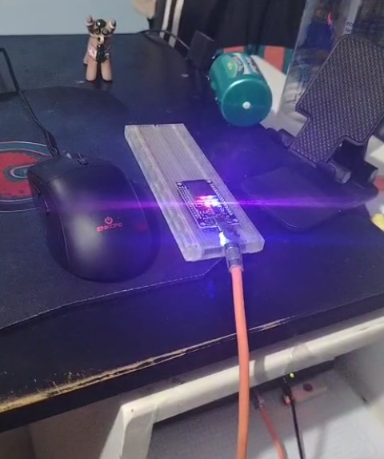
\includegraphics[width=\textwidth]{img/montaje_fisico_1.png}
        \caption{Estado inicial / Reposo con LED activo.}
        \label{fig:fisico1}
    \end{subfigure}
    \hfill
    \begin{subfigure}[b]{0.48\textwidth}
        \centering
        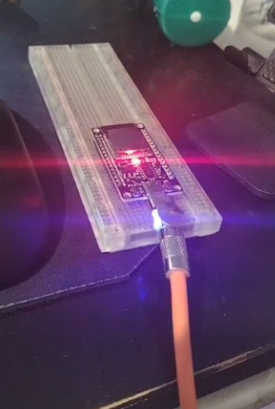
\includegraphics[width=\textwidth]{img/montaje_fisico_2.png}
        \caption{Transición y conmutación de estado.}
        \label{fig:fisico2}
    \end{subfigure}
    \caption{Evidencia experimental del montaje físico sobre protoboard en banco de trabajo.}
    \label{fig:montajes_fisicos}
\end{figure}

\section{Desarrollo y Resultados de las Simulaciones}

% ------------------------------------------------------------------------------
\subsection{Circuito 1: Prender y Apagar un LED (Blink)}
\textbf{Objetivo:} Generación de una señal periódica de conmutación en el pin digital \texttt{D8} con frecuencia $f = 0.5\text{ Hz}$ ($1000\text{ ms}$ ON, $1000\text{ ms}$ OFF).

\begin{lstlisting}[language=C++, caption={Código fuente del Circuito 1 (\texttt{01\_Blink\_LED.ino})}]
const uint8_t PIN_LED = 8;
const unsigned long TIEMPO = 1000;

void setup() {
  Serial.begin(9600);
  pinMode(PIN_LED, OUTPUT);
}

void loop() {
  digitalWrite(PIN_LED, HIGH); // LED ON
  Serial.println(F("[ESTADO] LED ENCENDIDO (HIGH)"));
  delay(TIEMPO);
  digitalWrite(PIN_LED, LOW);  // LED OFF
  Serial.println(F("[ESTADO] LED APAGADO (LOW)"));
  delay(TIEMPO);
}
\end{lstlisting}

\begin{figure}[H]
    \centering
    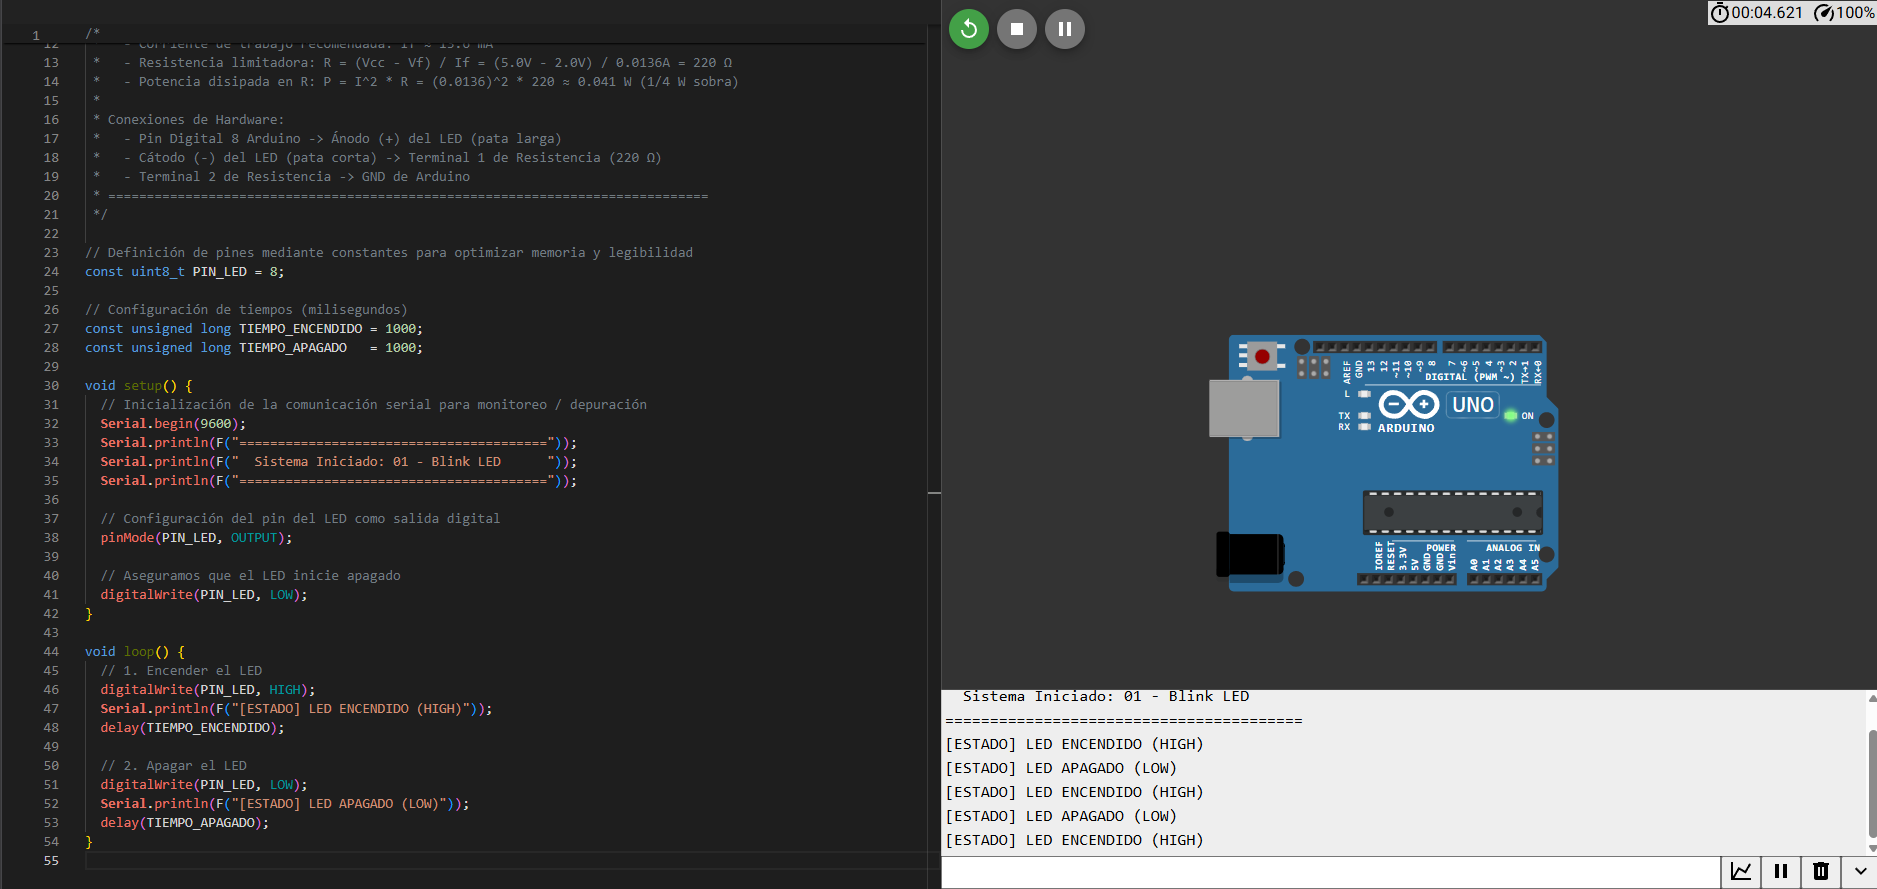
\includegraphics[width=0.88\textwidth]{img/circuito_1_wokwi.png}
    \caption{Simulación ejecutada del Circuito 1 en Wokwi mostrando el monitor serial y conmutación del LED.}
    \label{fig:sim1}
\end{figure}

% ------------------------------------------------------------------------------
\subsection{Circuito 2: Semáforo Americano (MUTCD)}
\textbf{Objetivo:} Implementar la secuencia cíclica vehicular regulada por el estándar estadounidense (\textit{Manual on Uniform Traffic Control Devices}): \textbf{Verde (5s) $\to$ Amarillo (2s) $\to$ Rojo (5s) $\to$ Verde}. A diferencia del esquema europeo, no se activa la combinación simultánea Rojo+Amarillo al arrancar.

\begin{table}[H]
\centering
\caption{Matriz de Estados del Semáforo Americano}
\label{tab:estados_americano}
\begin{tabular}{lcccc}
\toprule
\textbf{Fase} & \textbf{Pin D10 (Verde)} & \textbf{Pin D9 (Amarillo)} & \textbf{Pin D8 (Rojo)} & \textbf{Duración} \\
\midrule
1. Tránsito Libre & \textbf{HIGH} & LOW & LOW & 5.0 s \\
2. Advertencia & LOW & \textbf{HIGH} & LOW & 2.0 s \\
3. Alto Total & LOW & LOW & \textbf{HIGH} & 5.0 s \\
\bottomrule
\end{tabular}
\end{table}

\begin{figure}[H]
    \centering
    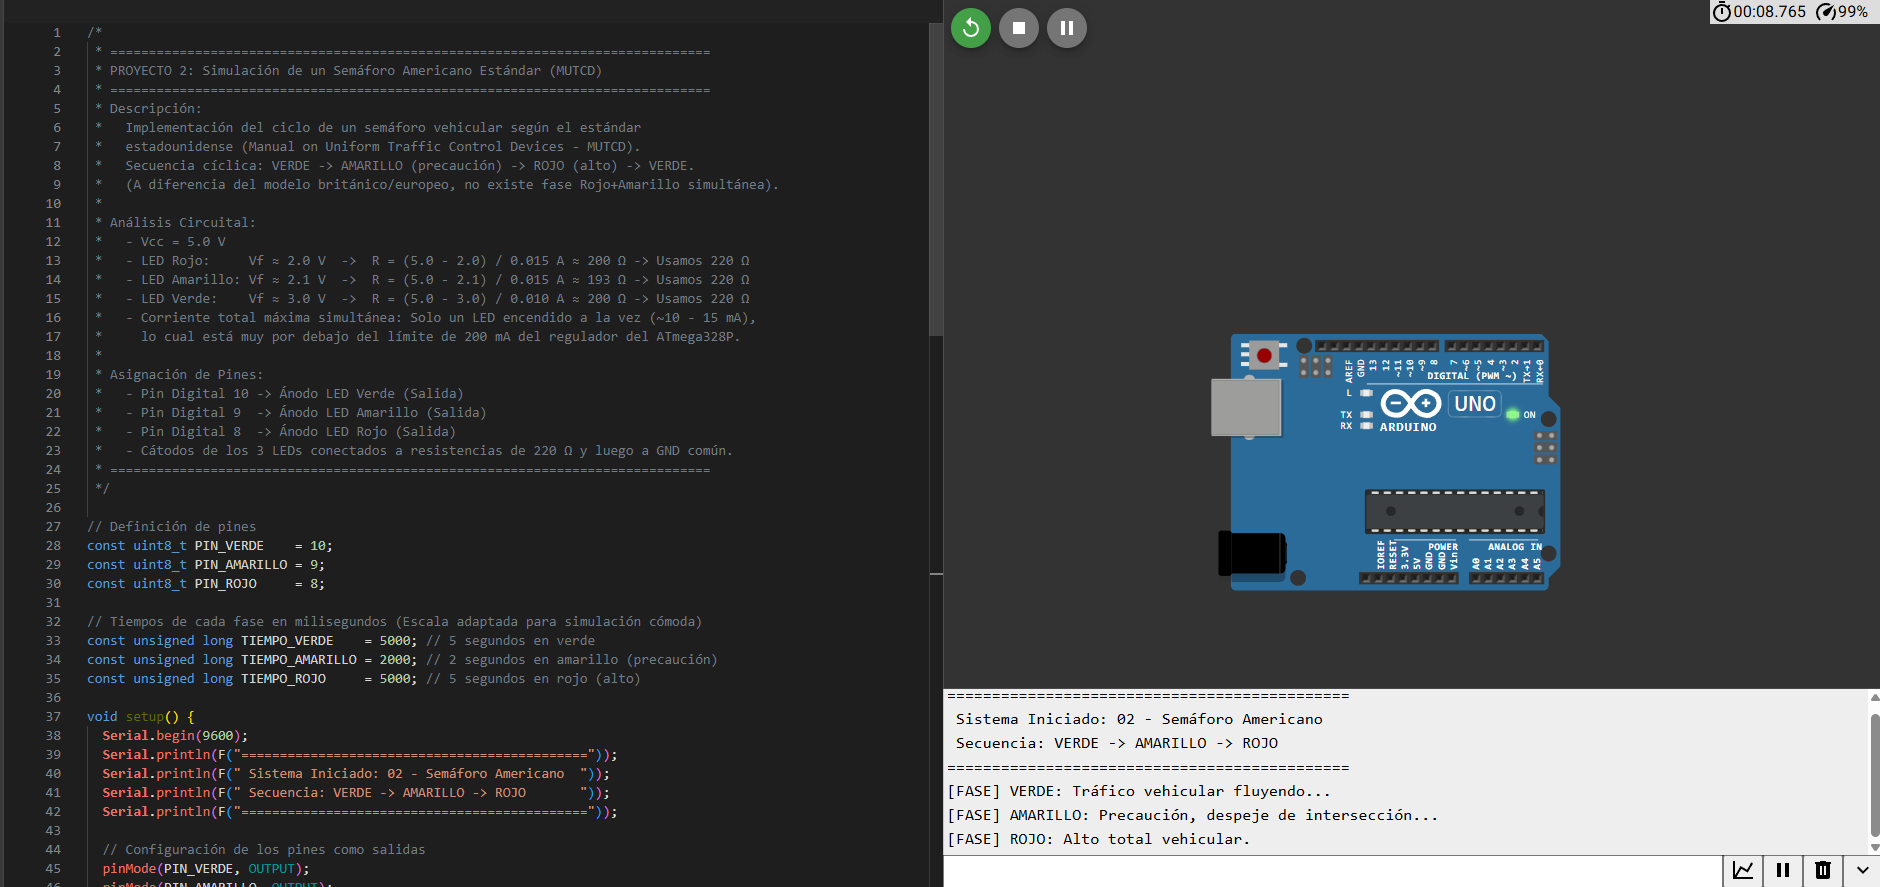
\includegraphics[width=0.88\textwidth]{img/circuito_2_wokwi.png}
    \caption{Simulación ejecutada del Semáforo Americano en Wokwi con logs de sincronización serial.}
    \label{fig:sim2}
\end{figure}

% ------------------------------------------------------------------------------
\subsection{Circuito 3: Semáforo para Carros y Personas Sincronizado}
\textbf{Objetivo:} Coordinación de 5 canales digitales garantizando interbloqueo estricto (exclusión mutua entre paso vehicular y peatonal), ventana de seguridad \textit{All-Red} de $1\text{ s}$ para evacuación de la intersección y destello de advertencia en el verde peatonal ($2\text{ s}$) antes del retorno a rojo.

\begin{table}[H]
\centering
\caption{Sincronización de Fases Vehicular vs Peatonal}
\label{tab:estados_mixto}
\begin{tabularx}{\textwidth}{c c c c X}
\toprule
\textbf{Fase} & \textbf{Autos (D10, D9, D8)} & \textbf{Peatones (D7, D6)} & \textbf{Tiempo} & \textbf{Acción Operativa} \\
\midrule
\textbf{1} & \textbf{Verde} & \textbf{Rojo} & 5.0 s & Flujo vehicular habilitado. \\
\textbf{2} & \textbf{Amarillo} & \textbf{Rojo} & 2.0 s & Advertencia y frenado de autos. \\
\textbf{3} & \textbf{Rojo} & \textbf{Rojo} & 1.0 s & \textit{All-Red}: Despeje total de vía. \\
\textbf{4} & \textbf{Rojo} & \textbf{Verde} & 4.0 s & Cruce peatonal seguro. \\
\textbf{5} & \textbf{Rojo} & \textbf{Verde (Destello)} & 2.0 s & Aviso de conclusión de cruce. \\
\textbf{6} & \textbf{Rojo} & \textbf{Rojo} & 1.0 s & Transición previa a verde vehicular. \\
\bottomrule
\end{tabularx}
\end{table}

\begin{figure}[H]
    \centering
    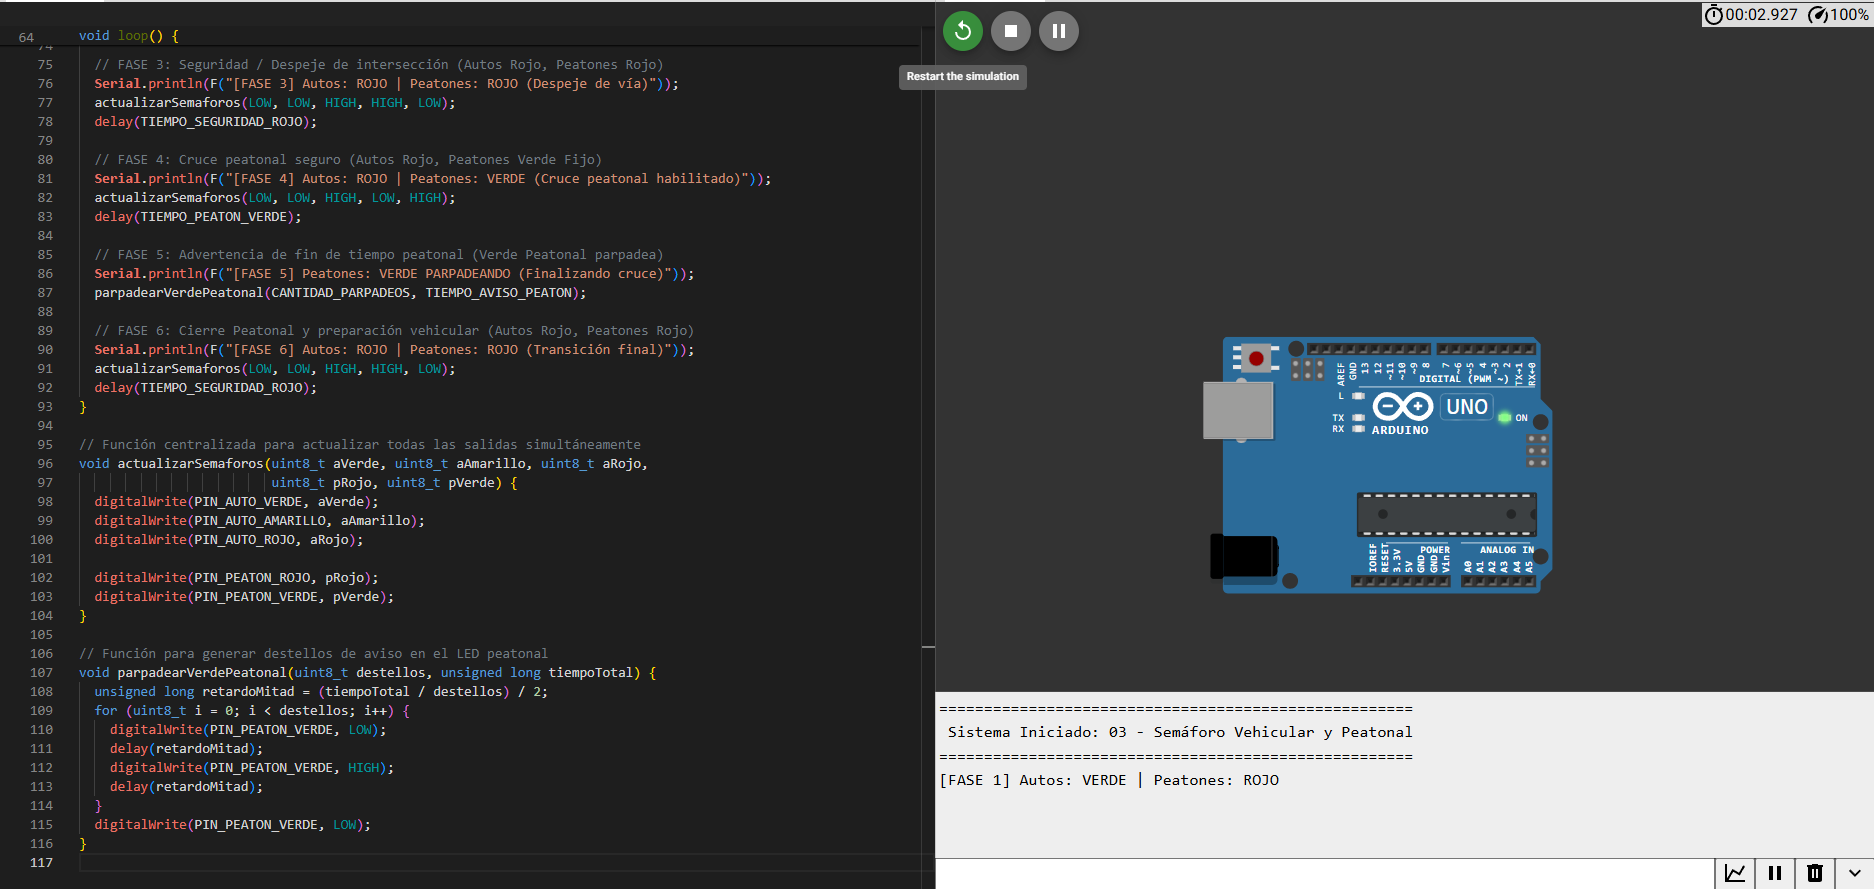
\includegraphics[width=0.88\textwidth]{img/circuito_3_wokwi.png}
    \caption{Simulación ejecutada del Semáforo Mixto en Wokwi evidenciando la alternancia entre autos y personas.}
    \label{fig:sim3}
\end{figure}

% ------------------------------------------------------------------------------
\subsection{Circuito 4: Semáforo con Botón Peatonal a Demanda (FSM No Bloqueante)}
\textbf{Objetivo:} Automatización reactiva a demanda mediante pulsador en pin digital \texttt{D2} con resistencia pull-up interna activada (\texttt{INPUT\_PULLUP}). Se implementa una **Máquina de Estados Finitos (FSM) no bloqueante** con \texttt{millis()} y filtro antirrebote (\textit{debounce}) de $200\text{ ms}$, asegurando un tiempo mínimo de verde vehicular de $4\text{ s}$ para evitar retenciones de tráfico ante pulsaciones consecutivas.

\begin{lstlisting}[language=C++, caption={Lógica no bloqueante y antirrebote del Circuito 4}]
void verificarBoton() {
  if (digitalRead(PIN_BOTON) == LOW) { // Flanco de bajada (presionado a GND)
    unsigned long ahora = millis();
    if (ahora - ultimoTiempoBoton >= TIEMPO_DEBOUNCE) {
      if (!peticionPeatonal && estadoActual == ESTADO_REPOSO_AUTO_VERDE) {
        peticionPeatonal = true;
        Serial.println(F("[EVENTO] Peticion peatonal registrada."));
      }
      ultimoTiempoBoton = ahora;
    }
  }
}
\end{lstlisting}

\begin{figure}[H]
    \centering
    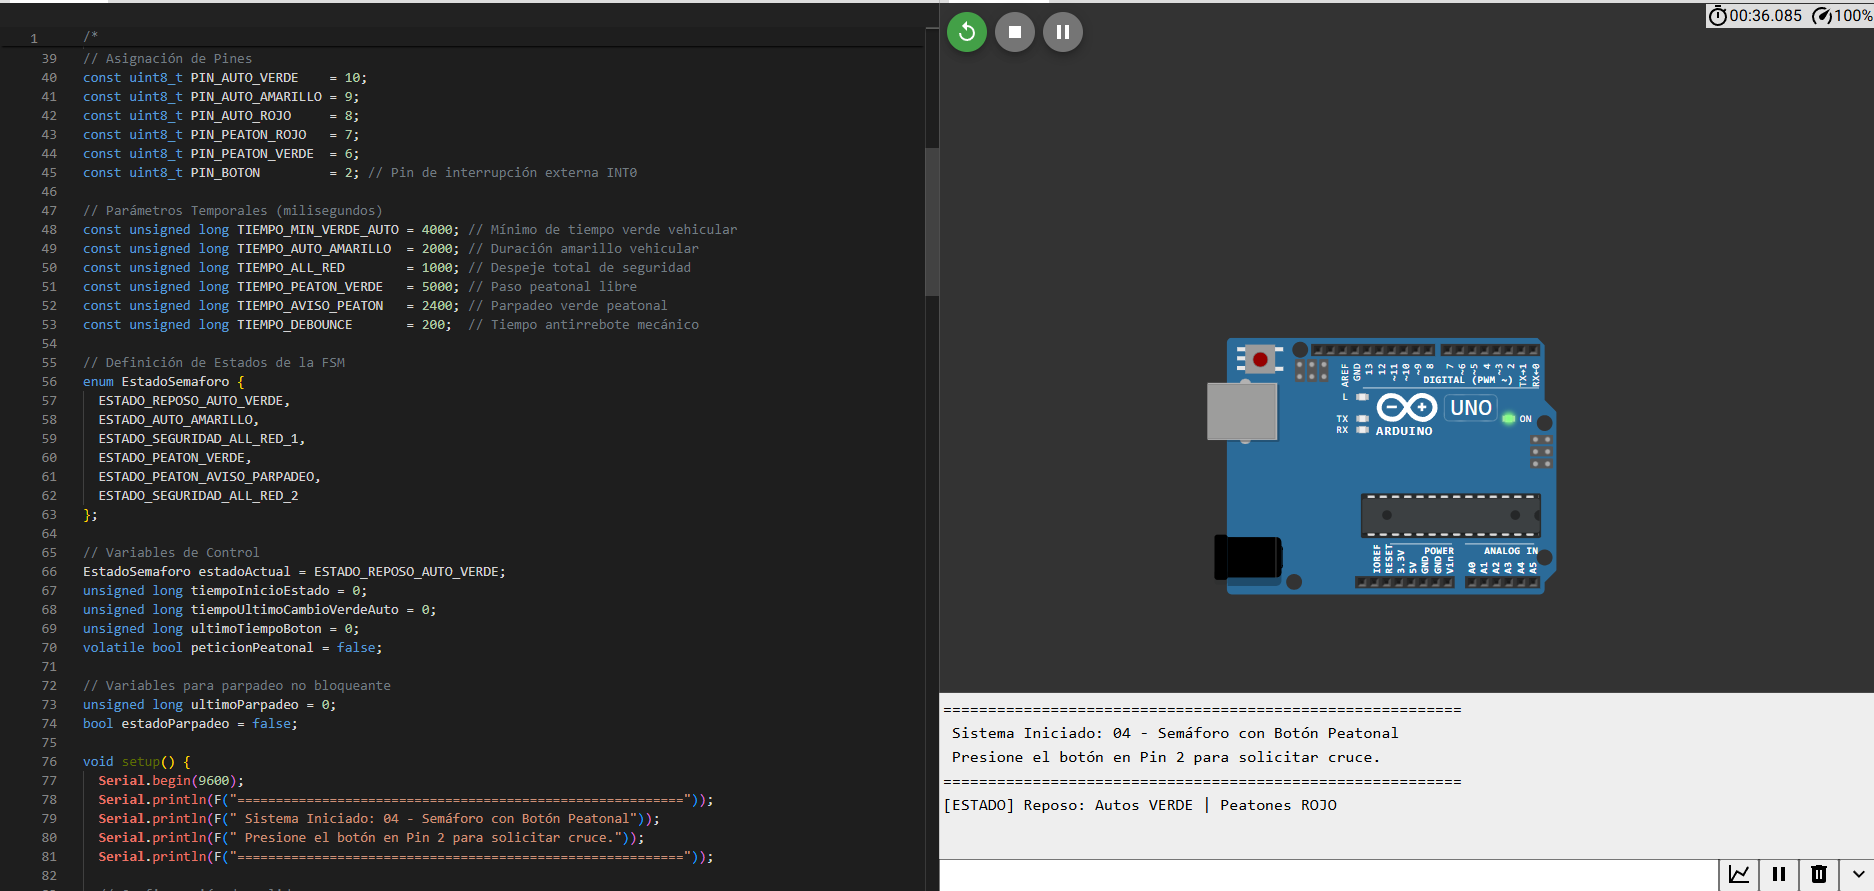
\includegraphics[width=0.88\textwidth]{img/circuito_4_wokwi.png}
    \caption{Simulación ejecutada del Semáforo Inteligente con Botón Peatonal en Wokwi y monitor serial.}
    \label{fig:sim4}
\end{figure}

\section{Comparativa de Resultados Experimentales}

\begin{table}[H]
\centering
\caption{Resumen Técnico Comparativo de los 4 Circuitos}
\label{tab:comparativa}
\begin{tabularx}{\textwidth}{l c c X c}
\toprule
\textbf{Proyecto} & \textbf{Salidas} & \textbf{Entradas} & \textbf{Arquitectura de Control} & \textbf{Consumo Máx.} \\
\midrule
01. Blink LED & 1 LED & 0 & Retardo Temporal Cíclico & 13.6 mA \\
02. Semáforo Americano & 3 LEDs & 0 & Secuencia 3 Fases MUTCD & 13.6 mA \\
03. Vehicular + Peatonal & 5 LEDs & 0 & Interbloqueo 6 Fases con \textit{All-Red} & 27.2 mA \\
04. Botón a Demanda & 5 LEDs & 1 Botón & FSM No Bloqueante (\texttt{millis()} + Debounce) & 27.2 mA \\
\bottomrule
\end{tabularx}
\end{table}

\section{Conclusiones}
\begin{enumerate}
    \item \textbf{Cálculo y Protección Circuital:} La elección del resistor limitador de $220\ \Omega$ mediante la Ley de Ohm garantiza una corriente de operación óptima de $13.6\text{ mA}$, operando en una zona segura respecto al límite del microcontrolador ($40\text{ mA}$).
    \item \textbf{Seguridad Vial en Sistemas Embebidos:} La integración de periodos \textit{All-Red} y parpadeos de fin de cruce asegura la integridad del peatón y elimina riesgos de colisión por cruces simultáneos.
    \item \textbf{Ventajas de la Arquitectura FSM No Bloqueante:} El uso de \texttt{millis()} frente a \texttt{delay()} en el Circuito 4 elimina la latencia del sistema, permitiendo registrar eventos asíncronos en tiempo real con filtrado antirrebote eficiente.
    \item \textbf{Integración Dual Simulación y Hardware:} Se validó la correspondencia entre la simulación en Wokwi y la plataforma física sobre protoboard.
\end{enumerate}

\section{Referencias y Trazabilidad}
\begin{itemize}
    \item \textbf{Repositorio GitHub Oficial:} \url{https://github.com/milith0kun/robotica-semaforos}
    \item \textbf{Simulador Wokwi Online:} \url{https://wokwi.com/projects/new/arduino-uno}
    \item \textbf{Atmel Datasheet:} \textit{ATmega328P 8-bit AVR Microcontroller Datasheet}, Rev. 8161D.
    \item \textbf{FHWA:} \textit{Manual on Uniform Traffic Control Devices (MUTCD)}, U.S. Dept. of Transportation.
    \item \textbf{ID de Sesión de Desarrollo:} \texttt{231cda85-c992-4f6b-8f80-94698b1b354a}
\end{itemize}

\end{document}
